%%% Local Variables:
%%% mode: latex
%%% TeX-master: t
%%% End:
\documentclass[serif ,mathserif ,professionalfont,hyperref={pdfpagelabels=false}]{beamer}
%\usepackage{lmodern}
\usepackage{exscale}
\usepackage{amsmath}
\usepackage{graphicx}
%\usepackage{mathptmx} % seems something to do with the font
\usepackage{helvet}
\usepackage{tcolorbox}
\usepackage{textpos}
\usepackage{xargs}
\usepackage{tikz}
\usepackage{amssymb}
\usepackage[]{algorithm2e}
\usepackage{pxfonts}
\usepackage{eulervm}
\usepackage[miktex]{gnuplottex} % for MiKTeX,`pdflatex -shell-escape`
                                % enabled
\usepackage[export]{adjustbox}
\usepackage{cite}
%\usepackage{gnuplottex} I have used this line to compile on TeXLive 2013
%\usepackage[pdftex,dvipsnames]{xcolor}
%\usepackage[colorinlistoftodos,prependcaption,textsize=tiny]{todonotes}
\usepackage{mathtools}
\DeclareMathOperator*{\argmin}{argmin}
\DeclareMathOperator*{\argmax}{argmax}

\renewcommand{\familydefault}{helvetica}
%\renewcommand{\labelitemi}{$\bluesquare$}
\newcommand{\labelitemi}{\textbf{\ding{192}}}
\newcommand{\localtextbulletone}{\textcolor{gray}{\raisebox{.45ex}{\rule{.6ex}{.6ex}}}}
\newcommand\norm[1]{\left\lVert#1\right\rVert}
\renewcommand{\labelitemi}{\localtextbulletone}
%\renewcommand\mathfamilydefault{\mathnormal}
%\renewcommand{\theequation}{\thechapter--\arabic{equation}} % for
                                % equation number style



\DeclareMathOperator{\dom}{dom}
\def\gdw{\mathrel{{>}\mkern-13mu{<}}}

\setbeamertemplate{itemize items}[square]


\usetheme{Frankfurt}
\setbeamercolor{section in head/foot}{fg=white, bg=blue!20!black!90}


%% commands definitions for
\newcommand\mynew{andyandyandy}

%% end of the definition of commands

%%% block definition
\newenvironment<>{redblock}[1]{%
  \setbeamercolor{block title}{fg=white,bg=red!75!black!65}%
  \setbeamercolor{block body}{fg=red!40!black!70,bg=red!60!black!20}%

  \begin{block}#2{#1}}{\end{block}}
\newenvironment<>{blueblock}[1]{%
  \setbeamercolor{block title}{fg=white,bg=blue!75!black!65}%
  \setbeamercolor{block body}{fg=black,bg=blue!60!black!20}%
  \begin{block}#2{#1}}{\end{block}}

\newenvironment<>{greyblock}[1]{%
  \setbeamercolor{block title}{fg=white,bg=black!75}%
  \setbeamercolor{block body}{fg=black,bg=black!40}%
  \begin{block}#2{#1}}{\end{block}}

\newenvironment<>{greenblock}[1]{%
  \setbeamercolor{block title}{fg=white,bg=green!75!black!65}%
  \setbeamercolor{block body}{fg=black,bg=green!60!black!20}%
  \begin{block}#2{#1}}{\end{block}}
%%% Block definition
\def\labelitemi{--}

% for the note style
% \newcommandx{\unsure}[2][1=]{\todo[linecolor=red,backgroundcolor=red!25,bordercolor=red,#1]{#2}}
% \newcommandx{\change}[2][1=]{\todo[linecolor=blue,backgroundcolor=blue!25,bordercolor=blue,#1]{#2}}
% \newcommandx{\info}[2][1=]{\todo[linecolor=OliveGreen,backgroundcolor=OliveGreen!25,bordercolor=OliveGreen,#1]{#2}}
% \newcommandx{\improvement}[2][1=]{\todo[linecolor=Plum,backgroundcolor=Plum!25,bordercolor=Plum,#1]{#2}}
% \newcommandx{\thiswillnotshow}[2][1=]{\todo[disable,#1]{#2}}

%% configuration for the slids style
\makeatletter
\setbeamertemplate{footline}
{
  \leavevmode%
  \hbox{%
    \begin{beamercolorbox}[wd=.333333\paperwidth,ht=2.25ex,dp=1.6ex,center]{author in head/foot}%
      \usebeamerfont{author in
        head/foot}%
      \insertshortauthor\hspace{1em}\beamer@ifempty{Advanced
        Topics in Computer Graphics}{}{Computer Graphics}
    \end{beamercolorbox}%
    \begin{beamercolorbox}[wd=.333333\paperwidth,ht=2.25ex,dp=1.6ex,center]{title in head/foot}%
      \usebeamerfont{title in head/foot}\insertshorttitle
    \end{beamercolorbox}%
    \begin{beamercolorbox}[wd=.333333\paperwidth,ht=2.25ex,dp=1.6ex,right]{date in head/foot}%
      \usebeamerfont{date in head/foot}\insertshortdate{}\hspace*{2em}
      \insertframenumber{} / \inserttotalframenumber\hspace*{2ex}
    \end{beamercolorbox}}%
  \vskip0pt%
}
\makeatother

\author[\parbox{.2\paperwidth}{}]{\bf Pan An }
\institute{National University of Singapore}
\title{Directional Dipole Model for Subsurface Scattering }

%% end of configuration




% \title{Convex Optimization}
% \author{Hu SiXing, Hakki Can Karaimer, Pan An, Philipp Keck}
%\date{Jan 20th, 2016}
\date{\today}
\setbeamertemplate{bibliography item}[triangle]
\begin{document}















\begin{frame}
  \titlepage
\end{frame}


%%% Local Variables:
%%% mode: latex
%%% TeX-master: "../main"
%%% End:
\newcommand{\flux}[1]{L_#1(\pmb{x}, \vec{\omega_o})}


\section{Introduction}

\begin{frame}
  \frametitle{Rendering Translucent Materials}
  \only<1>{\begin{figure}[!ht]
    \centering
    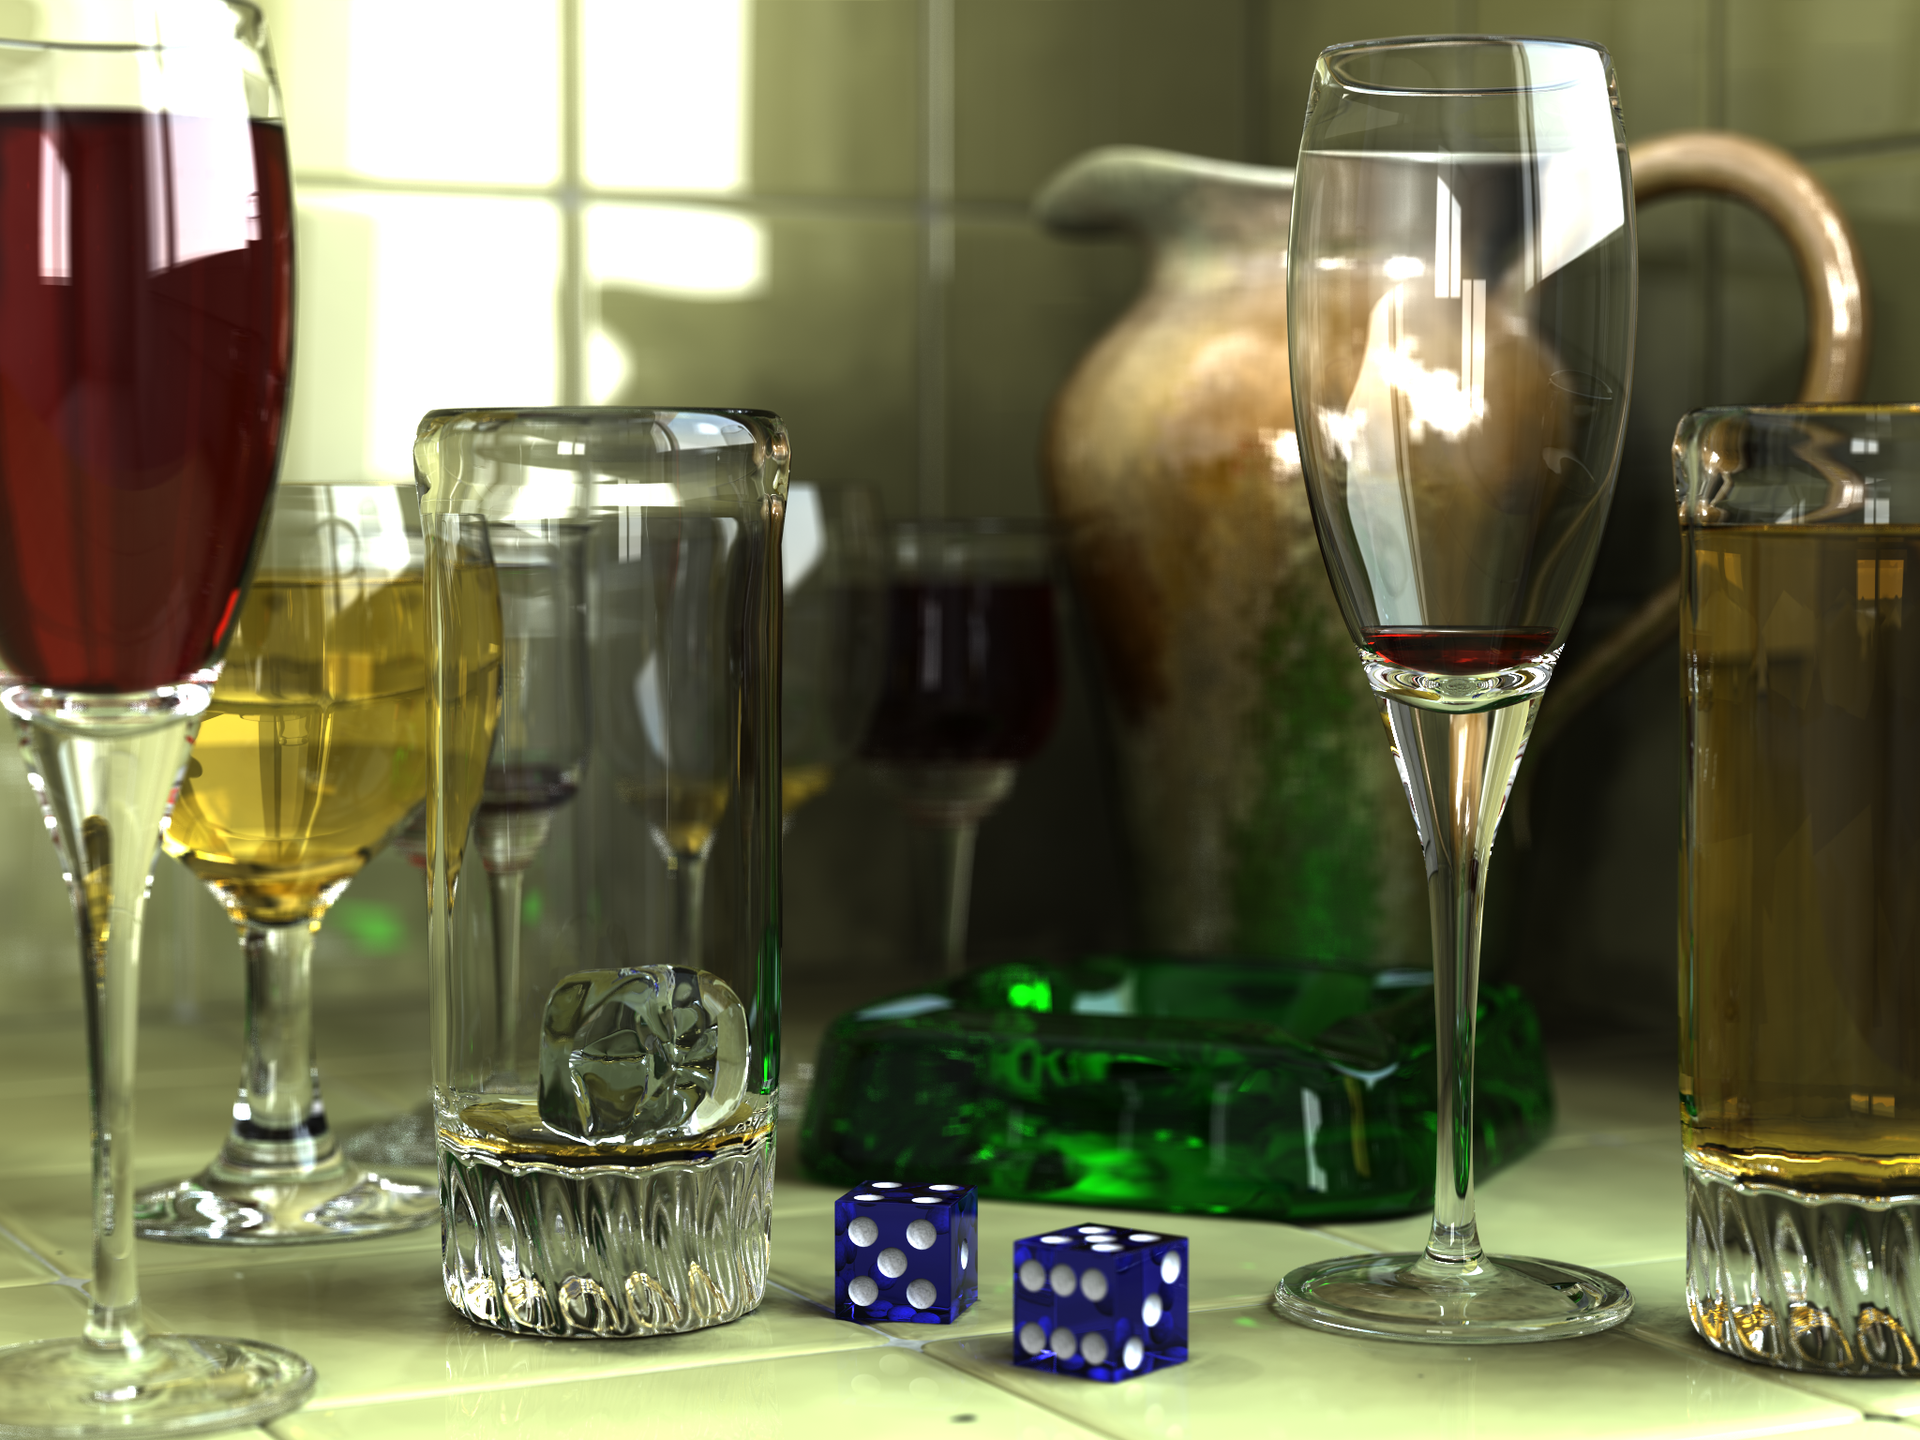
\includegraphics[scale=0.15]{renering.png}
  \end{figure}
}
\only<2>{
  \begin{figure}[!ht]
    \centering
    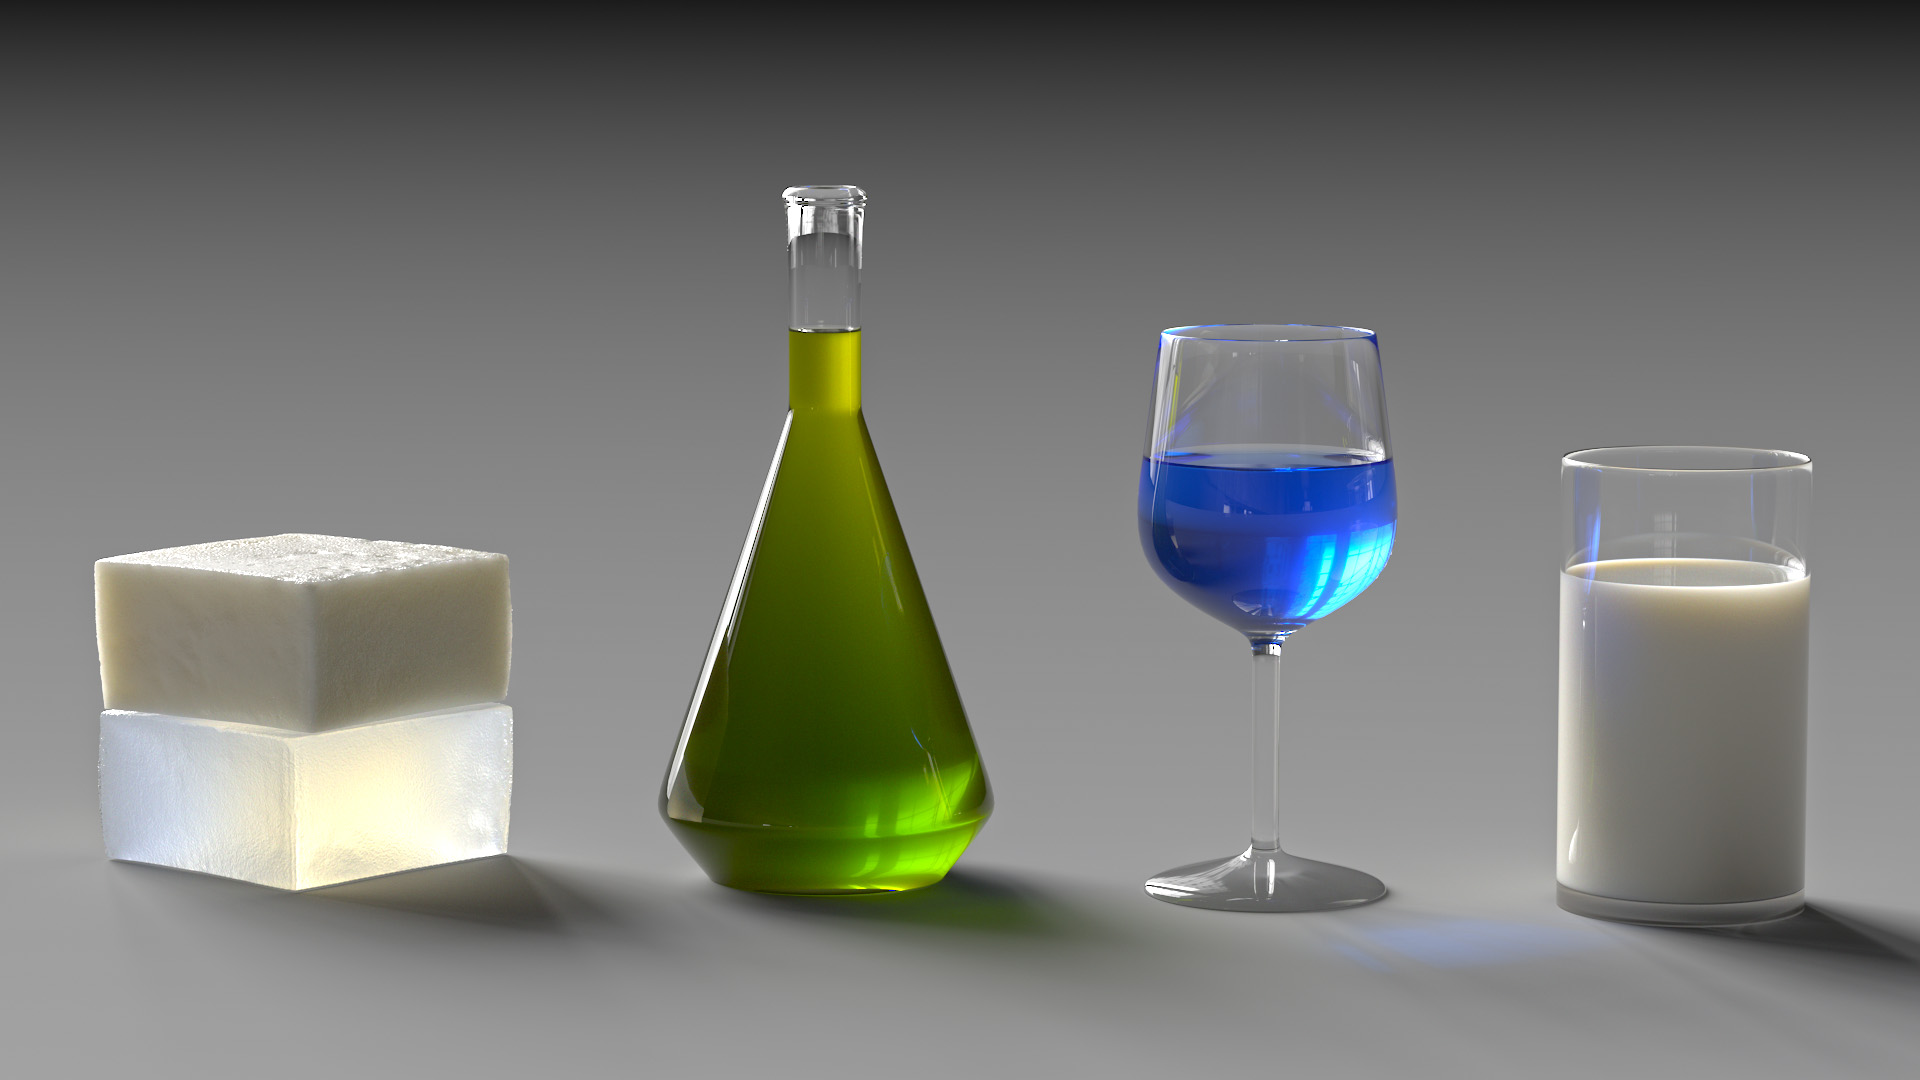
\includegraphics[scale=0.16]{trans.jpg}
  \end{figure}
}

\end{frame}


\section{BSSRDF}
\begin{frame}
  \frametitle{Light Transmission Models}
\only<1>{\begin{figure}[!ht]
    \centering
    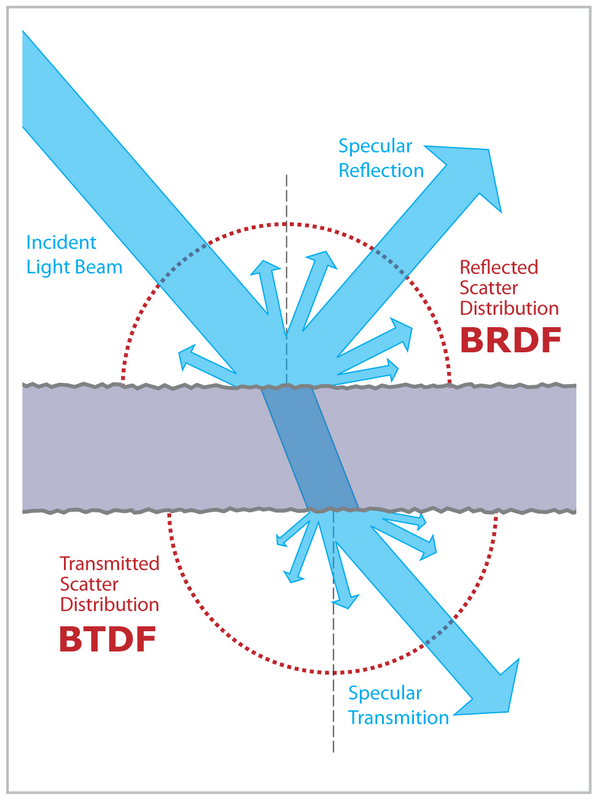
\includegraphics[scale=0.25]{bsdf.png}
  \end{figure}
}
\only<2>{
\begin{figure}[!ht]
    \centering
    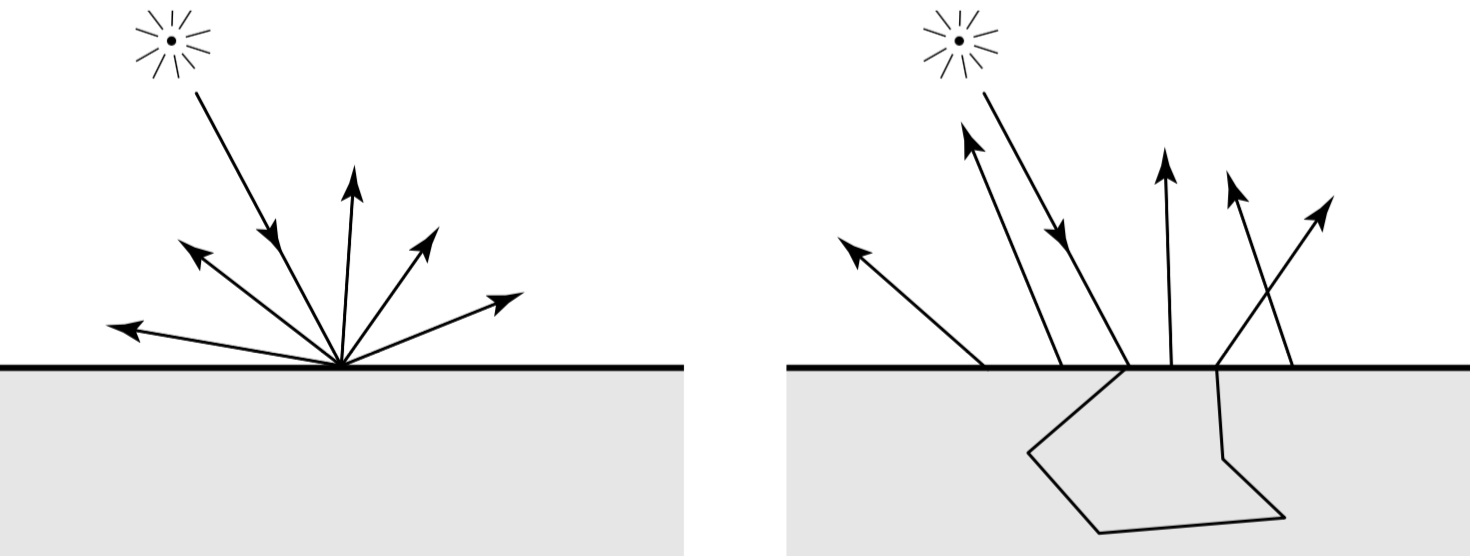
\includegraphics[scale=0.4]{bsdfbssrdf.png}
    \caption{Two models to describe the light transmission in
      translucent materials.}
  \end{figure}

}
\end{frame}





\begin{frame}
  \frametitle{BSSRDF Rendering}
Rendering translucent material takes a little bit more effort:

  \begin{align*}
\flux{o} &= \flux{e} + \flux{r} = \flux{e}\\
         & + \int_A\int_{2\pi}S(x_i, \vec{\omega_i}; x_o,
           \vec{\omega_o})L_i(\pmb{x}, \vec{\omega})(\vec{\omega}\cdot\vec{n})d\omega_idA
  \end{align*}

and

$$
S(x_i, \vec{\omega_i}; x_o, \vec{\omega_o})  = S_d(x_i,
\vec{\omega_i}; x_o, \vec{\omega_o}) +S^{(1)}(x_i, \vec{\omega_i};
x_o, \vec{\omega_o})
$$

where $S$ is BSSRDF. $S_d$ and $S^{(1)}$ are the{\bf  diffusion approximation} and
{\bf single scattering term}.

\end{frame}


\begin{frame}

\frametitle{Diffusion Approximation - Dipole}
  \begin{figure}[!ht]
    \centering
    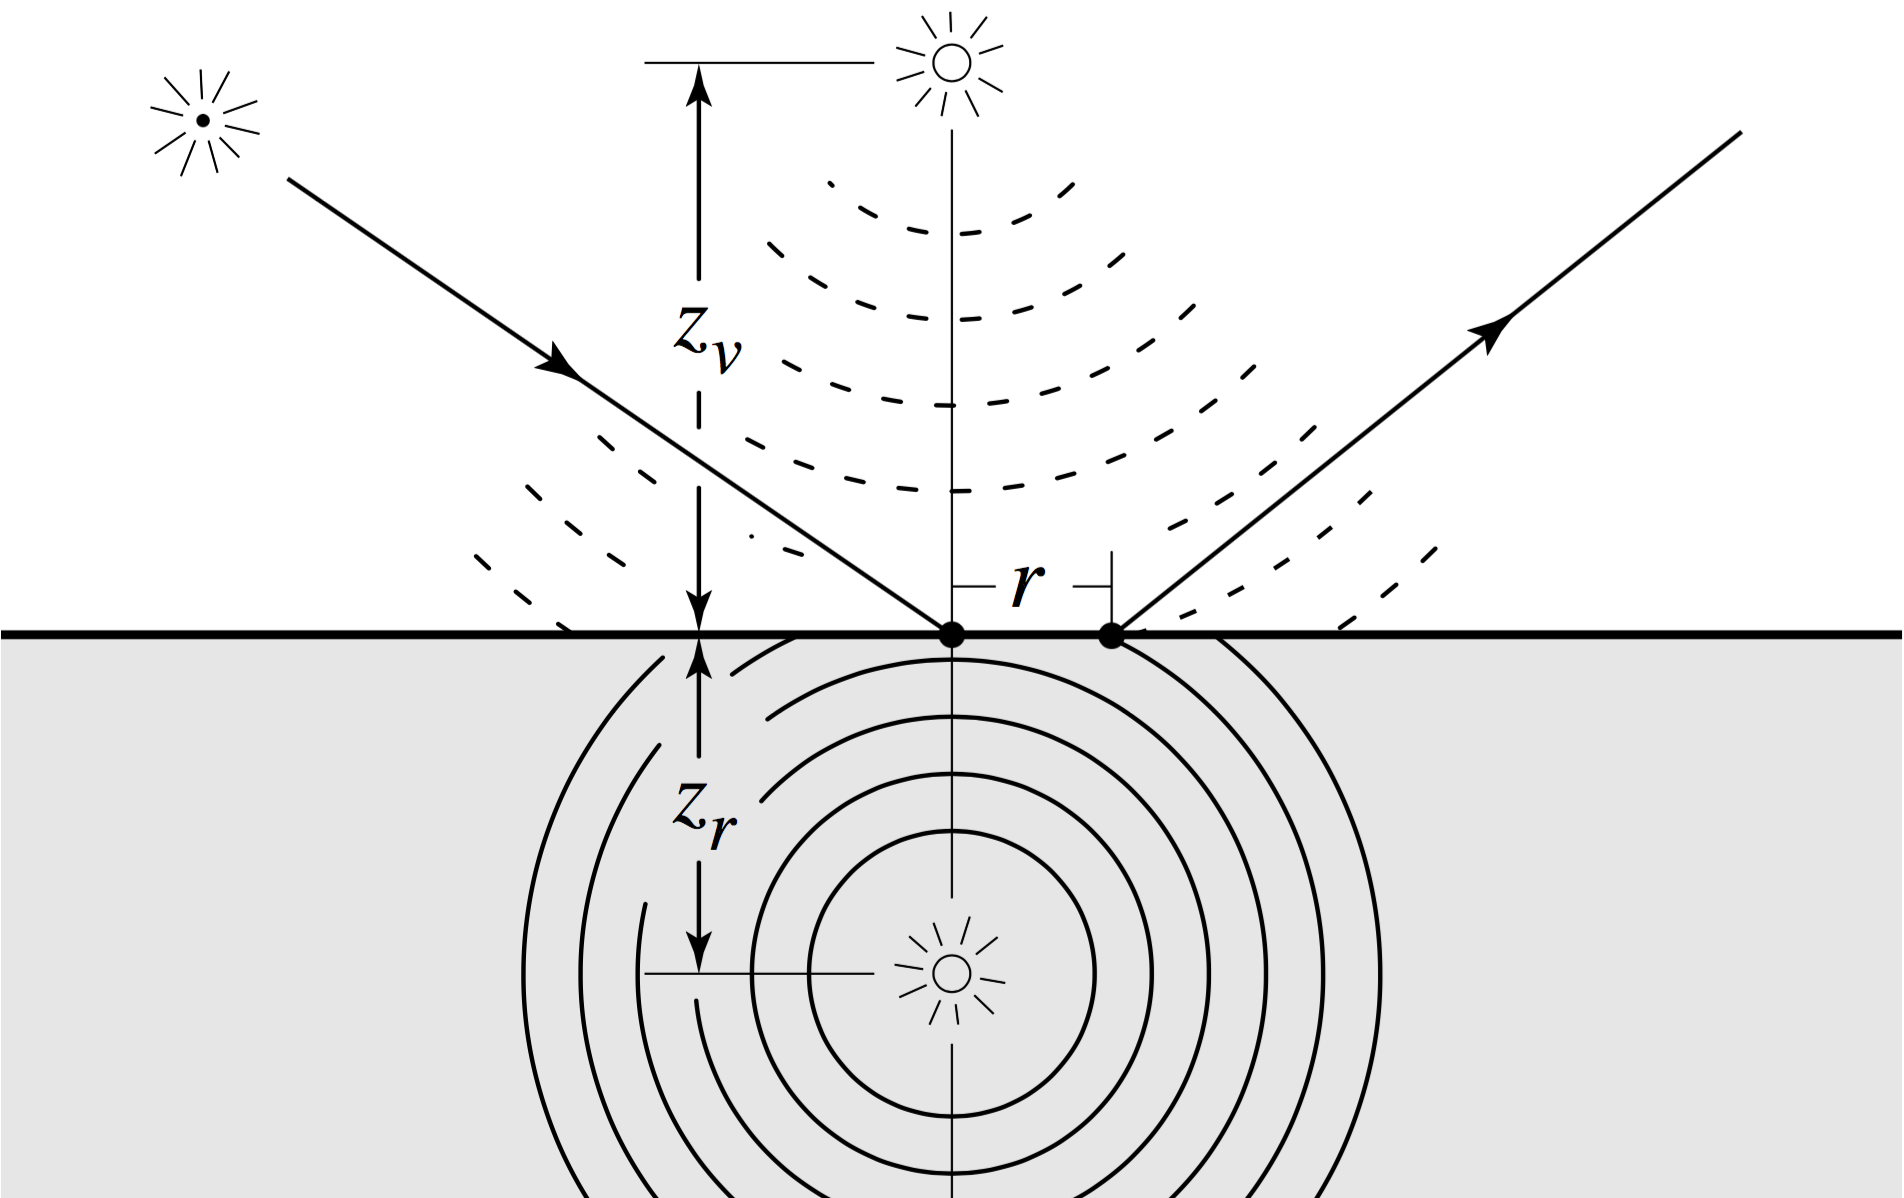
\includegraphics[scale=0.15]{di.png}
    \hspace{4mm}
    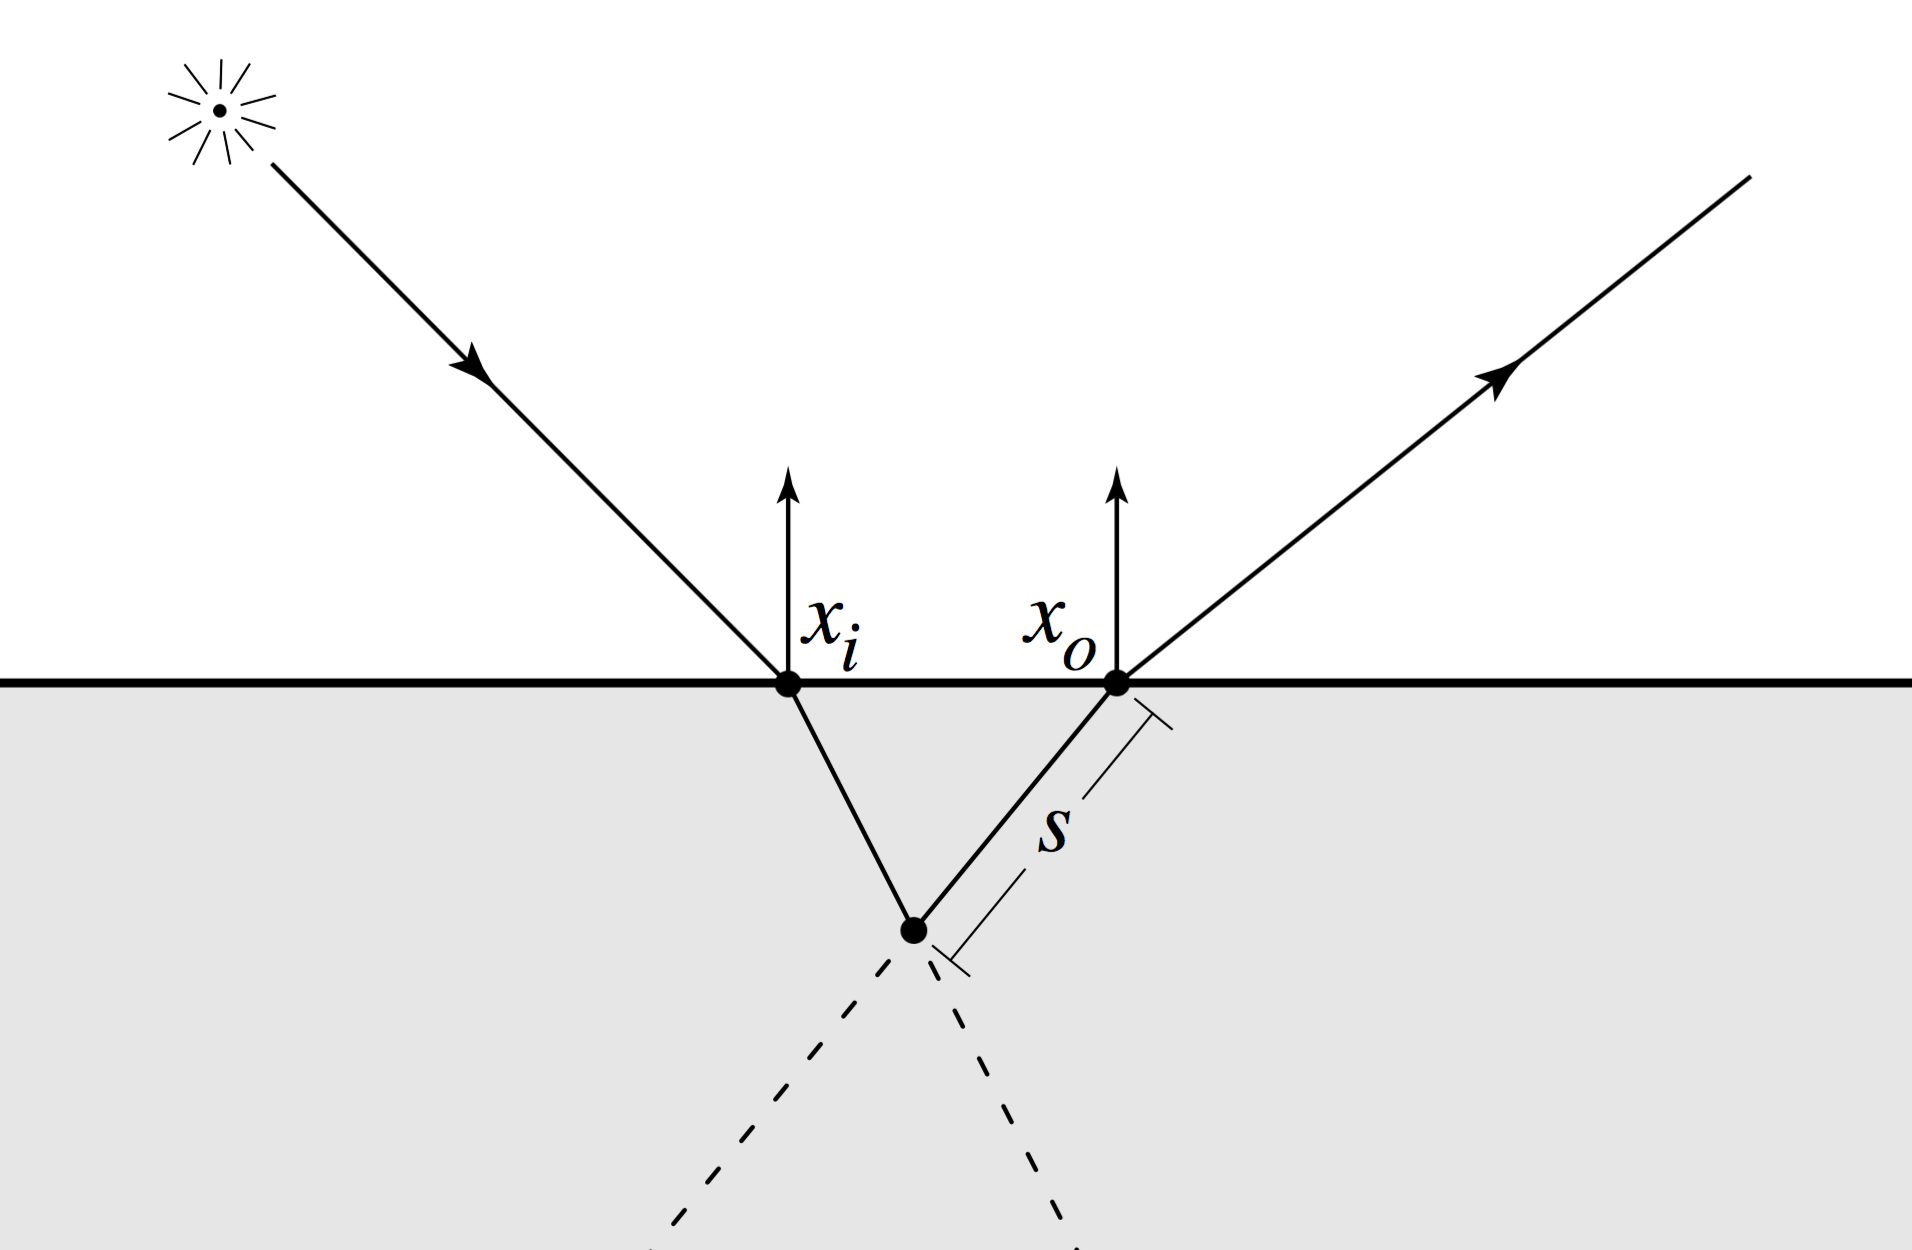
\includegraphics[scale=0.15]{single.png}
    \caption{A lot of math in the first graph. Single scattering occurs only when the refracted incoming and outgoing rays intersect.}
  \end{figure}
\end{frame}


\begin{frame}
  \frametitle{Photon Mapping - Engineering}
  \begin{itemize}
  \item Send photons to field, once intersecting with a surface, the
    incident(position and direction) will be stored in {\bf photon map};
  \item Actually 2 photon maps will be generated, one for caustics and
    one for SSS;
  \item Depends on the material, the action of the photon is processed
    with Monte Carlo method;
\item Then there should be optimizations, cause Monte Carlo is not
  graphic card friendly.
  \end{itemize}
\end{frame}




\section{Directional Dipole}

\begin{frame}
  \frametitle{Directional Dipole Model}
  \only<1>{\begin{figure}[!ht]
    \centering
    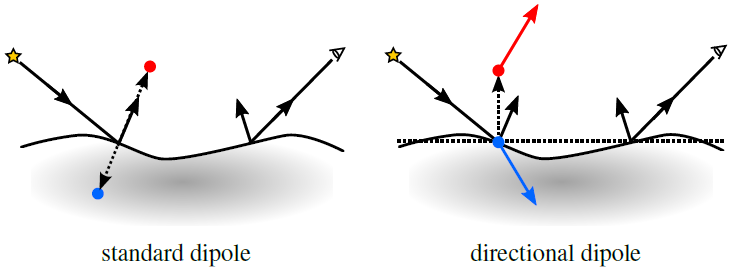
\includegraphics[scale=0.55]{dipoles.png}
  \end{figure}
}
\only<2>{
  \begin{figure}[!ht]
    \centering
    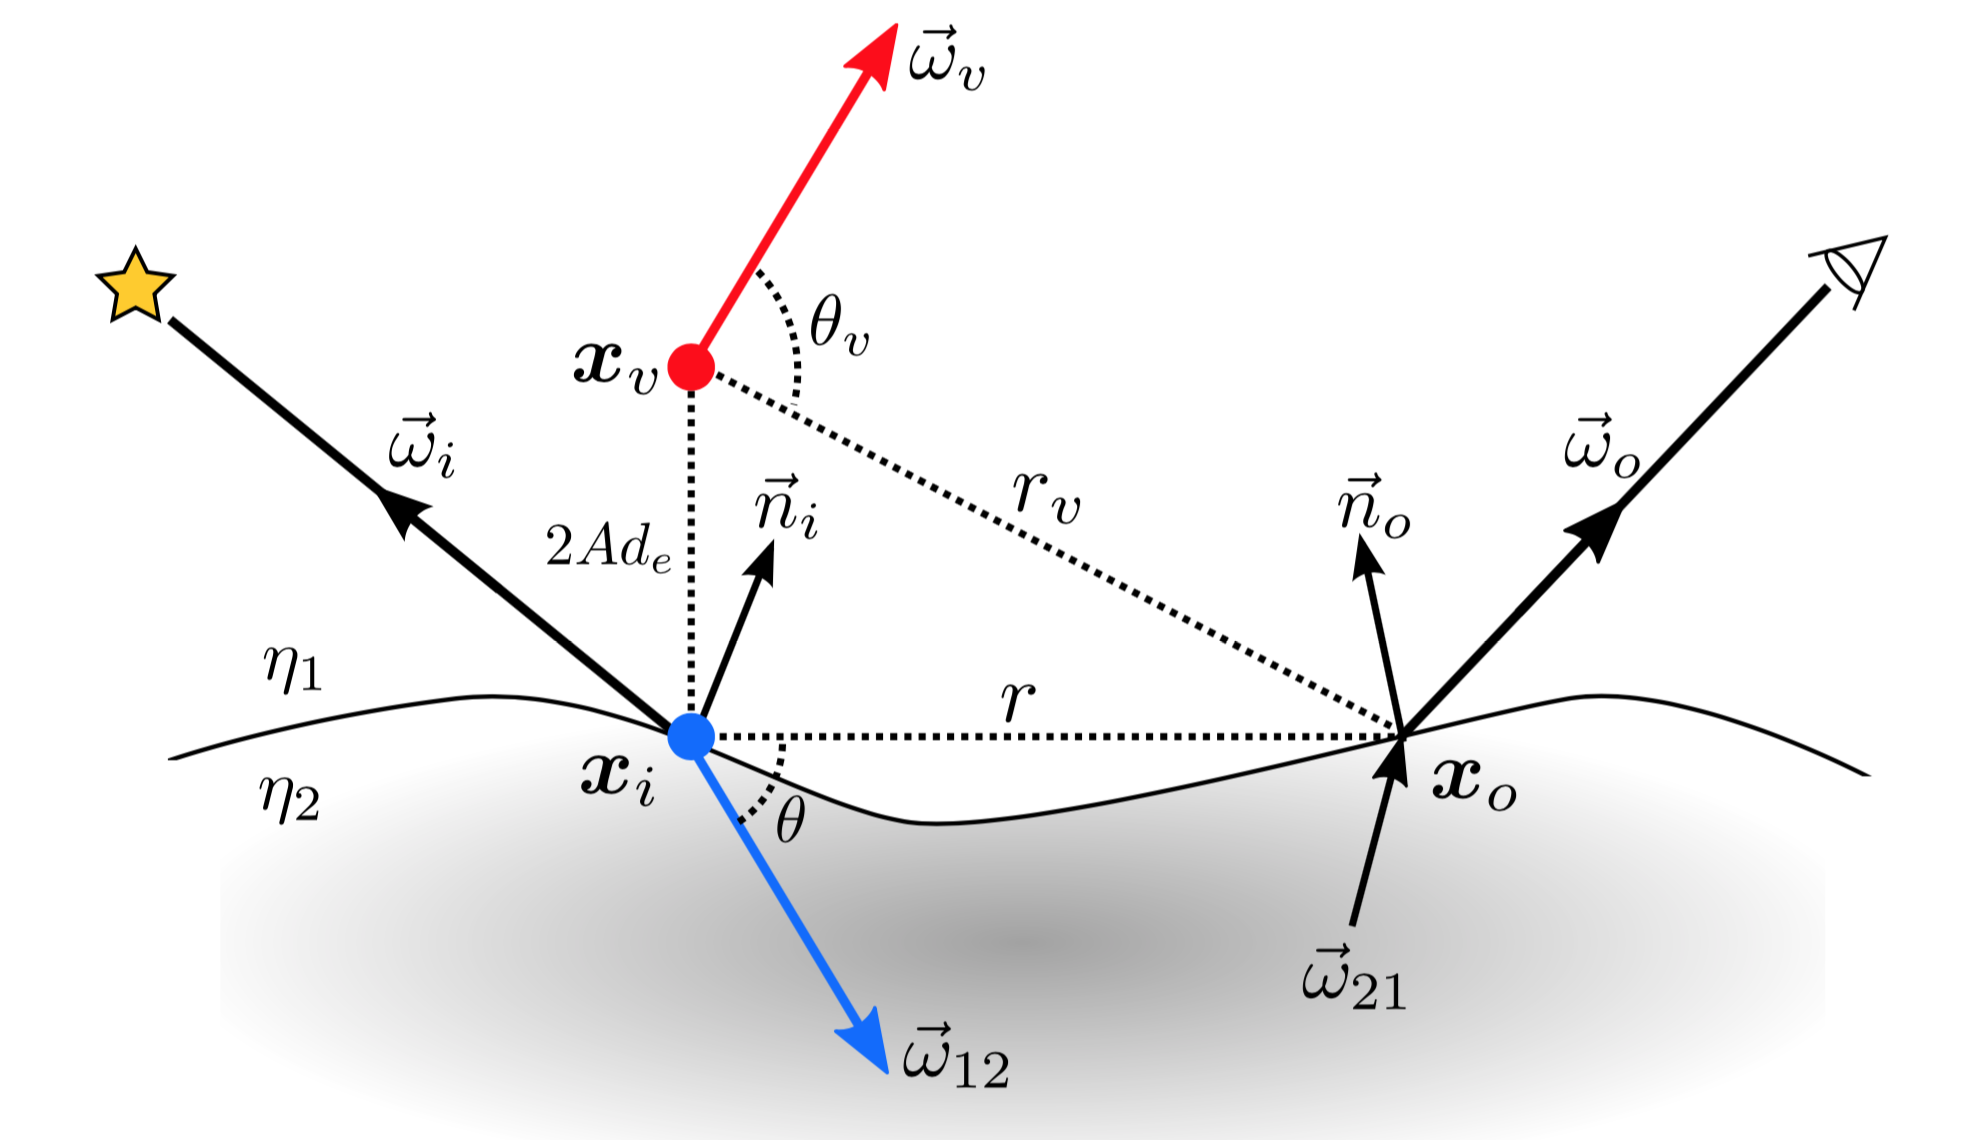
\includegraphics[scale=0.26]{direct.png}
  \end{figure}
And BSSRDF in this paper is(a lot of math):
$$
S_d(\pmb{x_i}, \vec{\omega}; \pmb{x_o}) = S'_d(\pmb{x_o - x_i},
\vec{\omega}_{12}, d_r) - S'_d(\pmb{x_o - x_v}, \vec{\omega}_{v}, d_v)
$$

}
\end{frame}

\begin{frame}
  \frametitle{Some Comparisons}
  \only<1>{
    \begin{figure}[!ht]
      \centering
      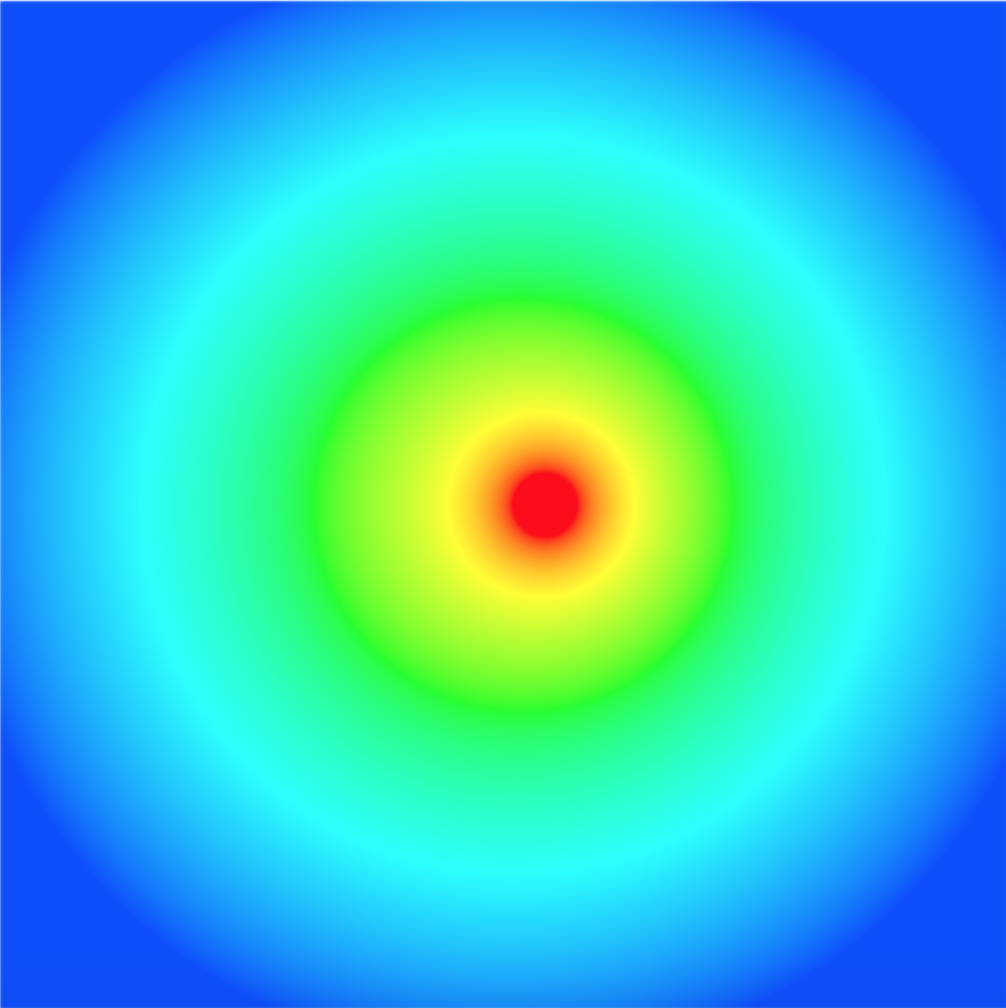
\includegraphics[scale=0.25]{so.png}
\hspace{4mm}
      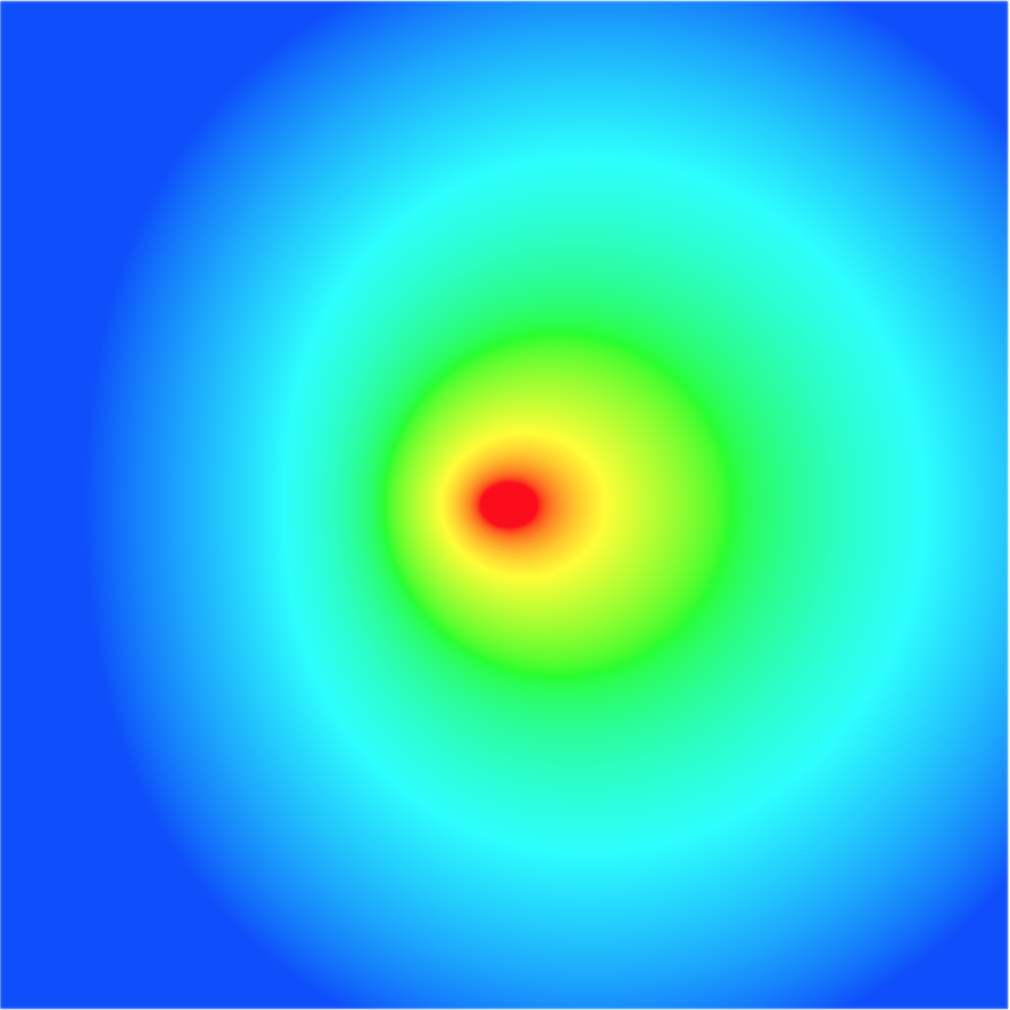
\includegraphics[scale=0.25]{sn.png}\\
    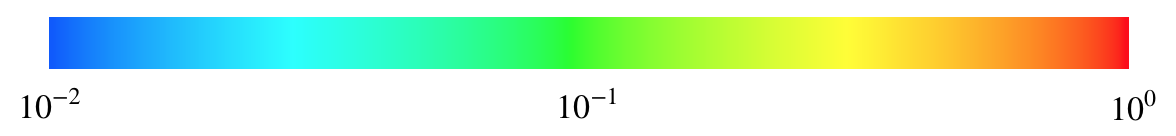
\includegraphics[scale=0.5]{bar.png}
      \caption{Diffuse reflectance due to approximate single
        scattering. Tested with Standard(left) and Directional Dipole. The
        incident angle is 45 degrees. }
    \end{figure}
  }
\only<2>{
\begin{figure}[!ht]
      \centering
      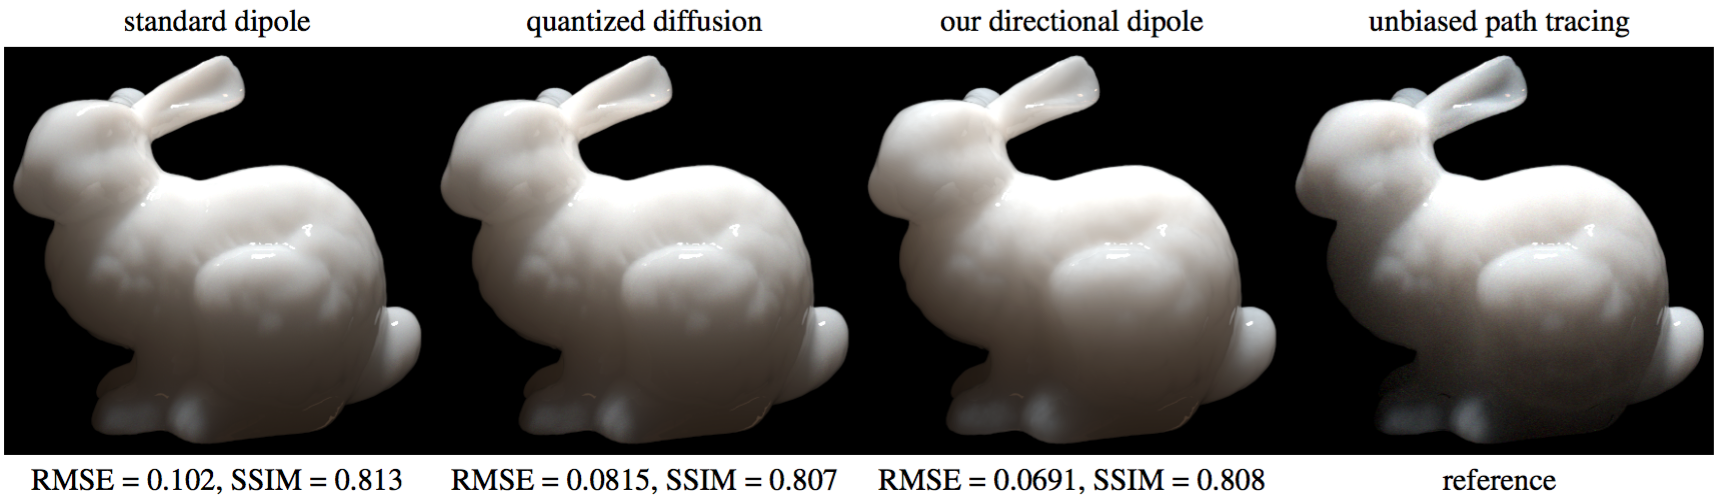
\includegraphics[scale=0.35]{stan.png}
      \caption{Comparison among different methods.}
    \end{figure}
}
\only<3>{
  \begin{itemize}
  \item No precomputation required;
  \item Single scattering does not need Monte Carlo simulation;
\item This whole thing is just to take the boundary into consideration actually.
  \end{itemize}
}
\end{frame}

\begin{frame}
  \frametitle{Basic Implementation}
  \begin{figure}[!ht]
    \centering
    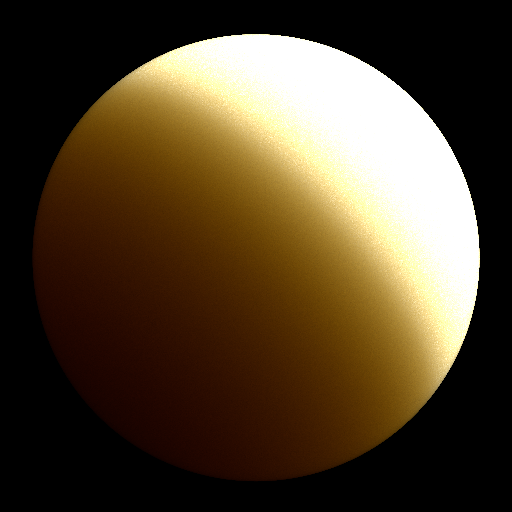
\includegraphics[scale=0.4]{render.png}
  \end{figure}
\end{frame}





\section{References}
\begin{frame}
  \frametitle{References}
\tiny

\nocite{*}
\bibliographystyle{plain}
\bibliography{papers}


\end{frame}




\end{document}


%%% Local Variables:
%%% mode: latex
%%% TeX-master: t
%%% End:
